\section{Training \ourmethod}
We pretrain \ourmethod following Alg. \ref{alg:pretraining} on several populations of trained NN models, from the model zoo dataset \citep{schurholtModelZoosDataset2022}. 
We use zoos of small models to compare with previous work, as well as zoos containing larger ResNet-18 models. 
All zoos are split into training, validation, and test splits $70:15:15$.
\vspace{-10pt}
\begin{itemize}
\item \textbf{Smaller CNN zoos.}
The MNIST and SVHN zoos contain LeNet-style models with 3 convolution and 2 dense layers and only $\sim 2.5k$ parameters. 
The slightly larger CIFAR-10 and STL-10 zoos use the same architecture with wider layers and $\sim 12k$ parameters.
\vspace{-6pt}
\item \textbf{Larger ResNet zoos.}
We also use the CIFAR-10, CIFAR-100, and Tiny-Imagenet zoos containing ResNet-18 models \citep{schurholtModelZoosDataset2022} with $\sim 12M$ parameters to evaluate scalability to large models. 
\end{itemize}

\vspace{-5pt}
\textbf{Pretraining.}
We train \ourmethod using Alg. \ref{alg:pretraining}.
As augmentations, we use noise and permutation. 
The permutation is computed relative to the aligned model. For contrastive learning, the aligned model serves as one view, and a permuted version as the second view. \looseness-1

\textbf{Implementation Details.} 
To maintain diversity within each batch, we select only a single window from each model. Loading, preprocessing, and augmenting the entire sample, only to use ca. 1\% of it, is infeasible. To address this, we leverage FFCV \citep{leclercFFCVAcceleratingTraining2023} to compile datasets consisting of sliced and permuted windows of models. Each model is super-sampled for approximately full coverage within the training set, considering the ratio of window length to sequence length.
For the ResNet zoos, we include 140 models per zoo, a number that remains manageable in terms of memory and storage. 
We train for 50 epochs using a OneCycle learning rate scheduler \citep{smithSuperConvergenceVeryFast2018}. Seeds are recorded to ensure reproducibility.
We build \ourmethod in PyTorch \citep{paszkePyTorchImperativeStyle2019}, using automatic mixed precision and flash attention \citep{daoFlashAttentionFastMemoryEfficient2022} to enhance performance. We use ray.tune \citep{liawTuneResearchPlatform2018} for hyperparameter optimization. 


%%%%%%%%%%%%%%%%%%%%%%%%%%%%%%%%%%%%%%%%%%%%%%%%%%%%%%%%%%%%%%%%%%%%%%%%%%%%%%%%%%%%%%%%%%%%%%%%%%%
\vspace{-4pt}
\section{Embedding Analysis}
\vspace{-2pt}
In this section, we analyze the embeddings of \ourmethod and compare to the weight-analysis methods \textit{WeightWatcher} (WW) \citep{martinPredictingTrendsQuality2021}. 
We focus on three aspects: 
i) global relation between accuracy and embeddings; 
ii) the trend of embeddings over layer index, as in  \citep{martinPredictingTrendsQuality2021}; and
iii) the identification of training phases as in \citep{martinTraditionalHeavyTailedSelf2019,martinImplicitSelfregularizationDeep2021}.
\vspace{-2pt}

To analyze weights, we focus on two WW metrics which in previous work reveal model performance as well as internal model composition (\textit{correlation flow}); the log spectral norm $\log(\| \mathbf{W}\|^2_{\infty})$ and weighted $\alpha$, the coefficient of the power law fitted to the empirical spectral density \citep{martinPredictingTrendsQuality2021}. 
These two metrics describe different aspects of the eigenvalue distribution. 
To get a similar signal on the internal dependency of weight matrices, we compute per-layer scalars $\hat{z}_l$ as the spread of the tokens of one layer in hyper-representation space, i.e., their standard deviation: 
\begin{align}
\vspace{-4pt}
    \hat{z}_l &=  std_t(\textbf{z}^t_m) \\
    \textbf{z}^t_m &= g(\textbf{W}^t_m),
\vspace{-4pt}
\end{align}
where $g$ is the hyper-rep encoder, $\textbf{z}^t_m$ are the stacked tokens $t$ of layer $m$, and $\textbf{W}^t_m$ is the weight-slice $t$ of layer $m$.
%
\vspace{-2pt}

To compare WW metrics to \ourmethod,
we pretrain \ourmethod on a Tiny-Imagenet ResNet-18 zoo and compute the two metrics on ResNets and VGGs of different sizes trained on ImageNet from pytorchcv \citep{semeryOsmrImgclsmob2024}.
On both ResNets in Figure \ref{fig:ww_comparison_layers_resnet}, \ref{fig:ww_comparison_layers_resnets_2x2} and VGGs in Figure \ref{fig:ww_comparison_layers_vgg}, the WW metrics and our embeddings show similar global trends. 
On ResNets, our embeddings and WW have low values at early layers and a sharp increase at the end. 
However, our embeddings add an additional step for intermediate layers, which may indicate that \ourmethod is sensitive to a higher degree of variation in these layers which previous work found by comparing activations \citep{kornblithSimilarityNeuralNetwork2019}.\looseness-1 

%%%%%%%%%%%%
\begin{figure}[h]
\centering
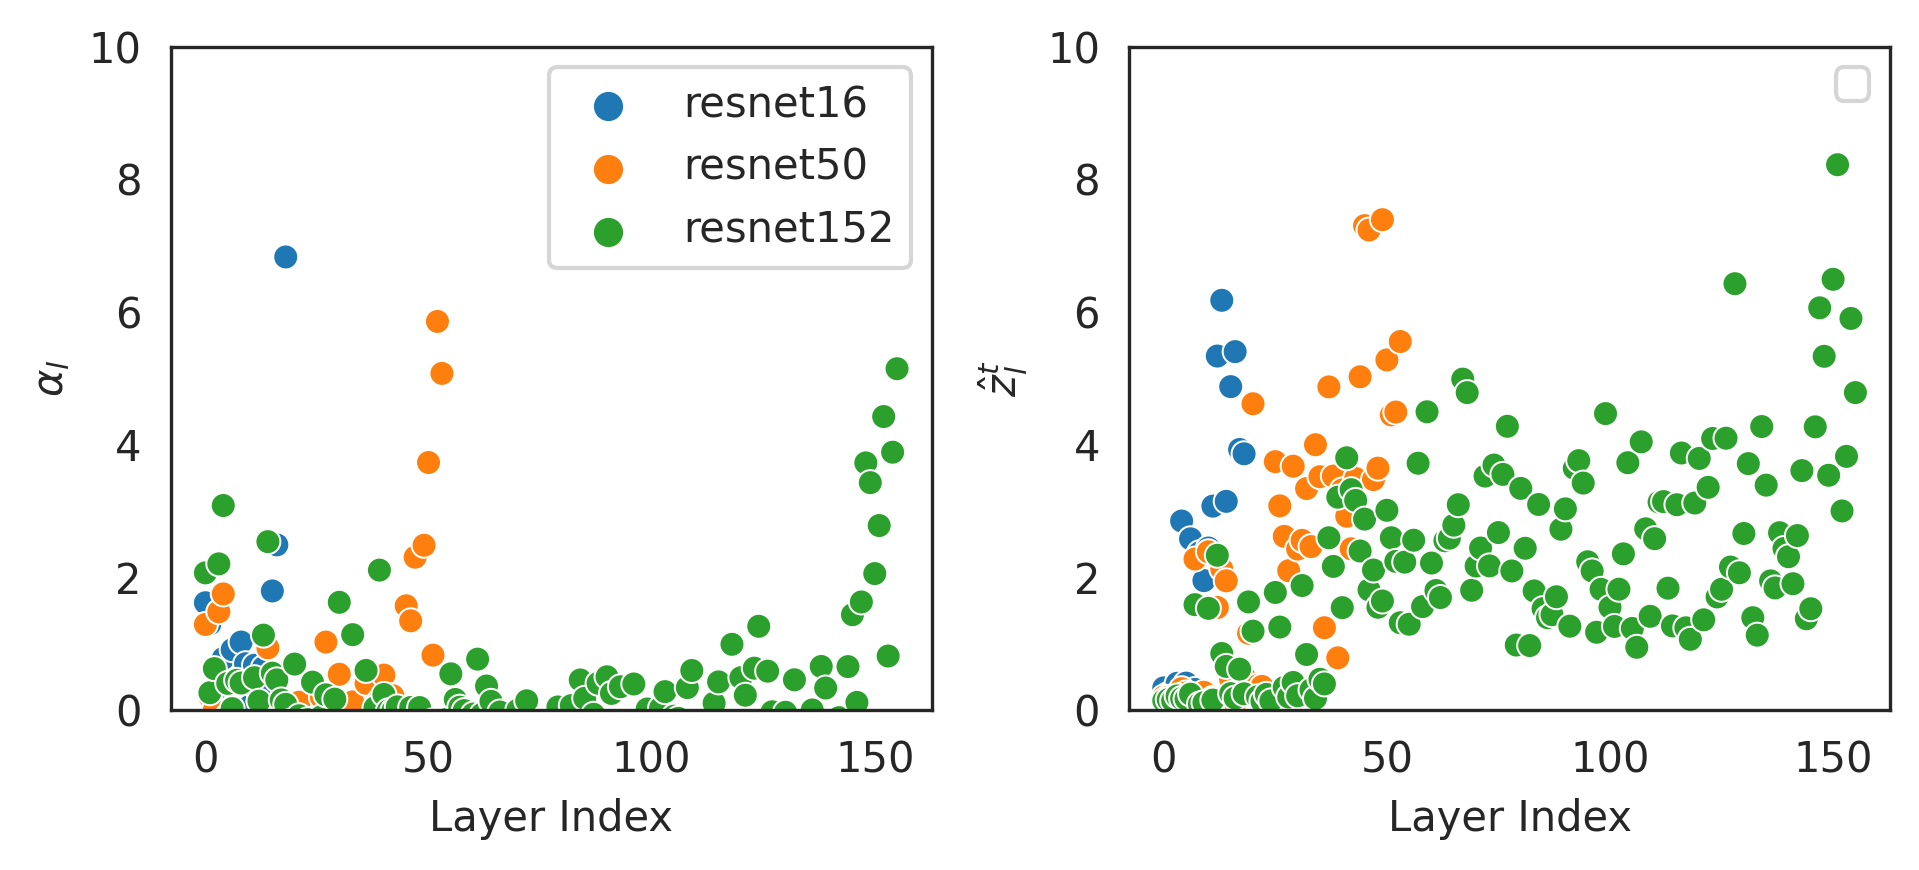
\includegraphics[trim=4mm 0mm 1.5mm 1.5mm, width=1.0\linewidth]{figures/ww_comparison_layers_2.png}
\vspace{-20pt}
\captionof{figure}{Comparison between WeightWatcher (WW) features (left) and \ourmethod (right). Features over layer index for ResNets from pytorchcv of different sizes.  
}
\vspace{-2mm}
\label{fig:ww_comparison_layers_resnet}
\end{figure}
%%%%%%%%%%%%
In a second experiment, we aggregate the layer-wise embeddings $\hat{z}_l$ to evaluate relations to model accuracy in Figures \ref{fig:ww_comparison_accuracy}, \ref{fig:ww_comparison_accuracy_2x2} and \ref{fig:ww_comparison_accuracy_our_zoo}, similar to previous work \citep{martinPredictingTrendsQuality2021}. 
On models from pytorchcv and the Tiny-ImagNet model zoo from \citep{schurholtModelZoosDataset2022}, the WW features and \ourmethod embeddings both show strong correlations to model accuracy. 
However, while the WW metrics are negatively correlated to accuracy, our embeddings are positively correlated to accuracy. 
The reason for that may lie in the additional 'step' in Figure \ref{fig:ww_comparison_layers_resnet}. 
That is, larger models with more layers generally have higher performance. As Figure \ref{fig:ww_comparison_layers_resnet} shows, more layers add very small values reducing the global average for WW metrics. For our embeddings, deeper models have more layers with higher $\hat{z}_l$ values, due to the afore-mentioned step. This increases the global model average with growing model size.
Lastly, we compare the eigenvalue spectrum to embeddings. Previous work identified distinct shapes at different training phases or with varying training hyperparameters  \citep{martinTraditionalHeavyTailedSelf2019,martinImplicitSelfregularizationDeep2021}. While we can replicate the distributions of the eigenvalues, the distributions of our embeddings only show the change from early phases of training to the heavy-tailed distribution; see Figure \ref{fig:ww_comparison_phases}. 

In summary, our embedding analysis indicates that \ourmethod represents several aspects of model quality (globally and on a layer level) that have been established previously.
% 
%%%%%%%%%%%%
\begin{figure}[h]
\centering
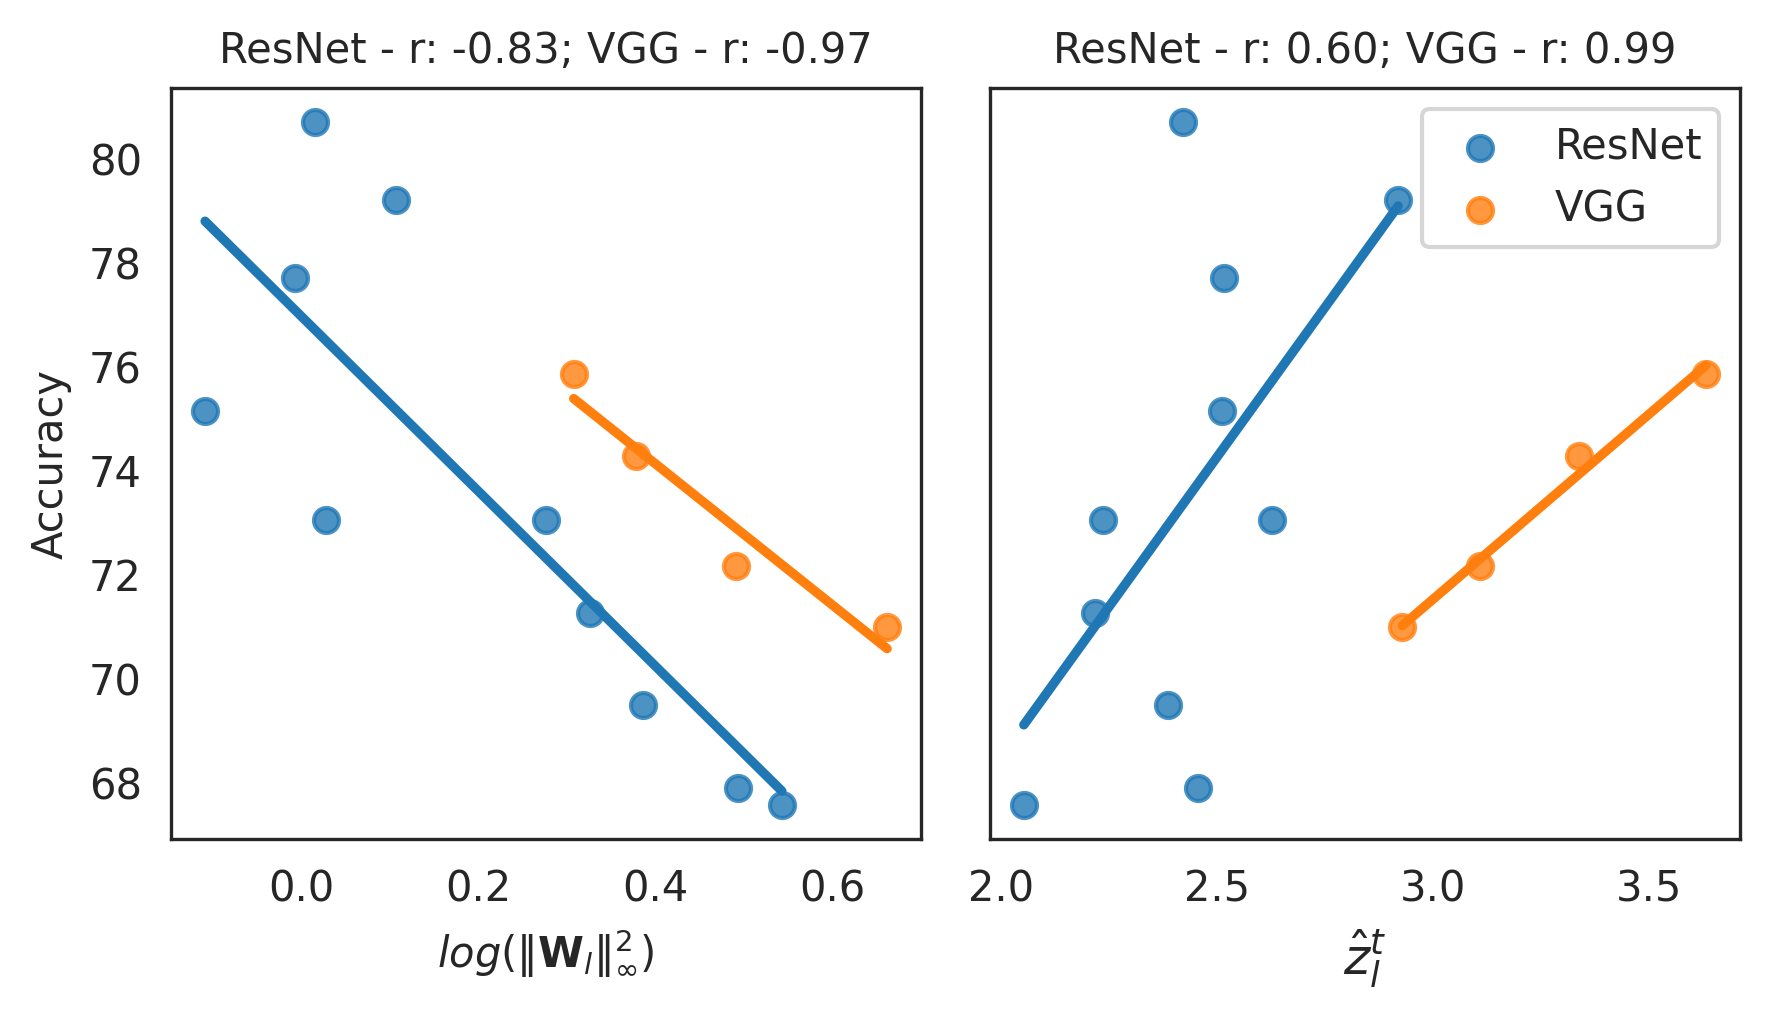
\includegraphics[trim={1mm 0mm 1.5mm 5.5mm}, clip, width=0.85\linewidth]{figures/ww_comparison_accuracy.png}
\vspace{-14pt}
\captionof{figure}{Comparison between WeightWatcher features (left) and \ourmethod (right). Accuracy over model features for ResNets and VGGs from pytorchcv of different sizes. Although \ourmethod is pretrained in a self-supervised fashion, it preserves the linear relation of a globally-aggregated embedding to model accuracy.
}
\vspace{-3mm}
\label{fig:ww_comparison_accuracy}    
\end{figure}
%%%%%%%%%%%%


%%%%%%%%%%%%%%%%%%%%%%%%%%%%%%%%%%%%%%%%%%%%%%%%%%%%%%%%%%%%%%%%%%%%%%%%%%%%%%%%%%%%%%%%%%%%%%%%%%%
\section{Empirical Performance}
In this section, we describe the general performance \ourmethod.
% 
\subsection{Predicting Model Properties}
\label{sec:property_prediction}
We evaluate \ourmethod for discriminative downstream tasks as a proxy for encoded model qualities. Specifically, we investigate whether \ourmethod matches the predictive performance of \textit{hyper-representations} on small CNN models (Table \ref{tab:discr_small_zoos}) and whether similar performance can be achieved on ResNet-18 models (Table \ref{tab:discr_resnet_zoos}). 
To that end, we compute model embeddings $\mathbf{\bar{z}}$ as outlined in Alg. \ref{alg:embeddings}, and we compare against flattened weights $W$ and weight statistics $s(W)$.
Following the experimental setup of \citep{eilertsenClassifyingClassifierDissecting2020,unterthinerPredictingNeuralNetwork2020,schurholtSelfSupervisedRepresentationLearning2021}, we compute embeddings using the three methods and linear probe for test accuracy (\texttt{Acc}), epoch (\texttt{Ep}), and generalization gap (\texttt{Ggap}). We again use trained models from the modelzoo repository \citep{schurholtModelZoosDataset2022}, with the same train, test, val splits as above. 
% 
\begin{table}[h]
\vspace{-4mm}
\captionof{table}{
Property prediction on populations of small CNNs used in previous work \citep{schurholtSelfSupervisedRepresentationLearning2021}. We report the regression $R^2$ on the test set prediction test accuracy \texttt{Acc.}, epoch \texttt{Ep.} and generalization gap \texttt{Ggap} for linear probing with model weights $W$, model weights statistics $s(W)$ or \ourmethod embeddings as inputs.\looseness-1}
\label{tab:discr_small_zoos}
\centering
\sc
\scriptsize
\setlength{\tabcolsep}{2.5pt}
\begin{tabularx}{1.0\linewidth}{lccccccccccc}
\toprule
      & \multicolumn{3}{c}{MNIST}                                                      &  & \multicolumn{3}{c}{SVHN}                                                       &  & \multicolumn{3}{c}{CIFAR-10 (CNN)}                                             \\ 
      \cmidrule(r){2-4} \cmidrule(lr){6-8} \cmidrule(lr){10-12}
      & \multicolumn{1}{c}{W} & \multicolumn{1}{c}{s(W)} & \multicolumn{1}{c}{\ourmethod} &  & \multicolumn{1}{c}{W} & \multicolumn{1}{c}{s(W)} & \multicolumn{1}{c}{\ourmethod} &  & \multicolumn{1}{c}{W} & \multicolumn{1}{c}{s(W)} & \multicolumn{1}{c}{\ourmethod}  \\ 
      \cmidrule(r){1-1} \cmidrule(r){2-4} \cmidrule(lr){6-8} \cmidrule(lr){10-12}
Acc.   & 0.965                 & \textbf{0.987}           & 0.978                       &  & 0.910                 & 0.985                    & \textbf{0.991}              &  & -7.580                & \textbf{0.965}           & 0.885                        \\
Ep. & 0.953                 & \textbf{0.974}           & 0.958                       &  & 0.833                 & \textbf{0.953}           & 0.930                       &  & 0.636                 & \textbf{0.923}           & 0.771                       \\
Ggap  & 0.246                 & 0.393                    & \textbf{0.402}              &  & 0.479                 & 0.711                    & \textbf{0.760}              &  & 0.324                 & \textbf{0.909}           & 0.772                       \\ 
\bottomrule
\end{tabularx}
\vspace{-2mm}
\end{table} 

\textbf{\ourmethod matches baselines on small models.}
The results of linear probing on small CNNs in Tables \ref{tab:discr_small_zoos} and \ref{tab:discr_small_zoos_full} confirm the performance of $W$ (low) and $s(W)$ (very high) of previous work. 
\ourmethod embeddings show comparably high performance to the $s(W)$ and previous \textit{hyper-representations}. 
Additional experiments in Appendix \ref{app:discr_comparison_previous_work} compare to previous work and confirm these findings. Sequential decomposition and representation learning as well as using the center of gravity does not significantly reduce the information contained in \ourmethod embeddings. 
%%%%%%%%%%%%%%%%%%%%%%%%%%%%%%%%%%%%%%%%%%%%%%%%%%%%%%%%%%%%%%%%%%%%%%%%%%%%%%%%%%%%%%%%%%%%%%%%%%%
%%%%%%%%%%%%%%%%%%%%%%%%%%%%%%%%%%%%%%%%%%%%%%%%%%%%%%%%%%%%%%%%%%%%%%%%%%%%%%%%%%%%%%%%%%%%%%%%%%%
% 
\begin{table}[h]
\vspace{-2mm}
\captionof{table}{
Property prediction on ResNet-18 model zoos of \citep{schurholtModelZoosDataset2022}. We report the regression $R^2$ on the test set prediction test accuracy \texttt{Acc.}, epoch \texttt{Ep.} and generalization gap \texttt{Ggap} for linear probing with model weights statistics $s(W)$ or \ourmethod embeddings as inputs.\looseness-1
}
\label{tab:discr_resnet_zoos}
\centering
\sc
\footnotesize
\setlength{\tabcolsep}{3.5pt}
\begin{tabularx}{1.0\linewidth}{lcccccccc}
\toprule
      & \multicolumn{2}{c}{CIFAR-10} &  & \multicolumn{2}{c}{CIFAR-100} &  & \multicolumn{2}{c}{Tiny-Imagenet} \\
      \cmidrule(){2-3} \cmidrule(){5-6} \cmidrule(){8-9} 
      &  s(W)     & \ourmethod    &  & s(W)     & \ourmethod    &      & s(W)      & \ourmethod      \\ 
\cmidrule(r){1-1} \cmidrule(){2-3} \cmidrule(){5-6} \cmidrule(){8-9} 
Acc.      & 0.880    & 0.879      &       & 0.923    & 0.922      &        &  0.802    &       0.795       \\
Ep.       & 0.999    & 0.999      &       & 0.999    & 0.992      &        &  0.999    &       0.980       \\
Ggap      & 0.490    & 0.512      &       & 0.882    & 0.879      &        &  0.704    &       0.699 
\\
\bottomrule
\end{tabularx}
\vspace{-4mm}
\end{table}

\newpage
\textbf{\ourmethod performance prediction scales to ResNets.} 
Both $s(W)$ and \ourmethod embeddings show similarly high performance on populations of ResNet-18s; see Table \ref{tab:discr_resnet_zoos}. 
On ResNet-18s, using the full weights $W$ for linear probing is infeasible due to the size of the flattened weights.
\ourmethod matches the high performance of $s(W)$. 
The results show that sequential \textit{hyper-representations} are capable of scaling to ResNet-18 models. 
Further, the aggregation even of long sequences (ca. 50k tokens) embedded in \ourmethod preserves meaningful information on model performance, which indicates the feasibility of applications like model diagnostics or targeted sampling.~\looseness-1
% 
%%%%%%%%%%%%%%%%%%%%%%%%%%%%%%%%%%%%%%%%%%%%%%%%%%%%%%%%%%%%%%%%%%%%%%%%%%%%%%%%%%%%%%%%%%%%%%%%%%%%%%%%%%%%%%%%%%%%%%%%%%%%%%%%%%%%%%%%%%%%%%%%%%%%%%%%%%%%%%%%%%%%%%%%%%%
% 
% 
\subsection{Generating Models}
\label{sec:generating_models}
We evaluate \ourmethod for the generative downstream tasks i.e., for sampling model weights. 
We generate weights following Alg. \ref{alg:generating} and test them in fine-tuning, transfer learning, and how they generalize to new tasks and architectures. 
In the following paragraphs, we begin with experiments on small CNN models from the modelzoo repository to compare with previous work (Tables \ref{tab:generative_cnn_zoos_in_domain}, \ref{tab:generative_cnn_zoos_transfer}). 
Subsequently, we evaluate \ourmethod for sampling ResNet-18 models for finetuning and transfer learning (Tables \ref{tab:generative_resnets_zoos_in_domain}, \ref{tab:generative_resnets_zoos_transfer}). 
Lastly, we evaluate sampling for new tasks and new architectures using only few prompt examples (Figure \ref{fig:sampling_new_arch_task} and Tables \ref{tab:generative_resnets_zoos_fewshot_transfer}, \ref{tab:generative_resnets_zoos_fewshot_resnet34}, \ref{tab:generative_resnets_zoos_fewshot_ti_resnet34}, \ref{tab:generative_resnets_zoos_fewshot_resnet34_one_prompt_example}).

We pretrain \ourmethod on models from the first half of the training epochs with Alg. \ref{alg:pretraining}, and keep the remaining epochs (26-50) as holdout to compare against, following the experimental setup of \citep{schurholtHyperRepresentationsGenerativeModels2022}. 
We sample using Alg. \ref{alg:generating} and use models from the last epoch in the pretraining set (epoch 25) as prompt examples. 
We denote subsampling with \ourmethod$_{SUB}$ and iteratively updating the distribution $\mathcal{P}$ as \ourmethod$_{BOOT}$. To evaluate the impact of the sampling method, we also combine \ourmethod with the $KDE30$ sampling approach that uses high-quality prompt examples \citep{schurholtHyperRepresentationsGenerativeModels2022}. We further evaluate sampling without prompt examples by bootstrapping off of a Gaussian prior $\mathcal{P}$, denoted as \ourmethod$_{GAUSS}$. We compare against training from scratch, as well as fine-tuning from the prompt examples.

%%%%%%%%%%%%%%%%%%%%%%%%%%%%%%%%%%%%%%%%%%%%%%%%%%%%%%%%%%%%%%%%%%%%%%%%%%%%%%%%%%
%%%%%%%%%%%%%%%%%%%%%%%%%%%%%%%%%%%%%%%%%%%%%%%%%%%%%%%%%%%%%%%%%%%%%%%%%%%%%%%%%%%%%%%%%%%%%%%

\begin{table}[t]
\vspace{-2mm}
\captionof{table}{
Model generation on CNN model populations fine-tuned on the same task. We compare training from scratch with $S_{KDE30}$ from \citep{schurholtHyperRepresentationsGenerativeModels2022}, \ourmethod combined with the $KDE30$ sampling method, and our \ourmethod subsampled. Each of the sampled populations is fine-tuned over 25 epochs.
}\label{tab:generative_cnn_zoos_in_domain}
\small
\setlength{\tabcolsep}{2.8pt}
\begin{tabularx}{1.0\linewidth}{clcccc}
\toprule
Ep.                  & \multicolumn{1}{c}{Method} & MNIST               & SVHN               & CIFAR-10           & STL                \\
\cmidrule(r){1-1} \cmidrule(lr){2-2} \cmidrule(lr){3-3} \cmidrule(lr){4-4} \cmidrule(lr){5-5} \cmidrule(l){6-6}
\multirow{5}{*}{0}     &  tr. fr. scratch                  & $\sim$10 /\%        & $\sim$10 /\%       & $\sim$10 /\%       & $\sim$10 /\%       \\
                       & $S_{KDE30}$                & 68.6$\pm$6.7           & 54.5$\pm$5.9          & \textit{n/a}                & \textit{n/a}                \\
                       & \ourmethod$_{KDE30}$                    & 84.8$\pm$0.8           & 70.7$\pm$1.4          & 56.3$\pm$0.5          & 39.2$\pm$0.8          \\
                       & \ourmethod$_{SUB}$                   & \textbf{86.7$\pm$0.8}  & \textbf{72.3$\pm$1.6} & \textbf{57.9$\pm$0.2} & \textbf{43.5$\pm$1.0} \\
                      & \ourmethod$_{GAUSS}$                 & 20.8$\pm$0.1                & 21.6$\pm$0.5                & 19.3$\pm$0.2               & 17.5$\pm$1.5               \\
\cmidrule(r){1-1} \cmidrule(lr){2-2} \cmidrule(lr){3-3} \cmidrule(lr){4-4} \cmidrule(lr){5-5} \cmidrule(l){6-6}
\multirow{5}{*}{1}     &  tr. fr. scratch                  & 20.6$\pm$1.6           & 19.4$\pm$0.6          & 37.2$\pm$1.4          & 21.3$\pm$1.6          \\
                       & $S_{KDE30}$                & 83.7$\pm$1.3           & 69.9$\pm$1.6          & \textit{n/a}                & \textit{n/a}                \\
                       & \ourmethod$_{KDE30}$                    & 85.5$\pm$0.8           & 71.3$\pm$1.4          & 58.2$\pm$0.2          & 43.5$\pm$0.7          \\
                       & \ourmethod$_{SUB}$                   & \textbf{87.5$\pm$0.6}  & \textbf{73.3$\pm$1.4} & \textbf{59.1$\pm$0.3} & \textbf{44.3$\pm$1.0} \\
                        & \ourmethod$_{GAUSS}$                 & 61.3$\pm$3.1                & 24.1$\pm$4.4                & 27.2$\pm$0.3               & 22.4$\pm$1.0               \\
\cmidrule(r){1-1} \cmidrule(lr){2-2} \cmidrule(lr){3-3} \cmidrule(lr){4-4} \cmidrule(lr){5-5} \cmidrule(l){6-6}
\multirow{5}{*}{5}     &  tr. fr. scratch                  & 36.7$\pm$5.2           & 23.5$\pm$4.7          & 48.5$\pm$1.0          & 31.6$\pm$4.2          \\
                       & $S_{KDE30}$                & \textbf{92.4$\pm$0.7} & 57.3$\pm$12.4         & \textit{n/a}                & \textit{n/a}                \\
                       & \ourmethod$_{KDE30}$                    & 87.5$\pm$0.7           & 72.2$\pm$1.2          & 58.8$\pm$0.4          & 45.2$\pm$0.6          \\
                       & \ourmethod$_{SUB}$                   & 89.0$\pm$0.4           & \textbf{73.6$\pm$1.5} & \textbf{59.6$\pm$0.3} & \textbf{45.3$\pm$0.9} \\
                       & \ourmethod$_{GAUSS}$                 & 83.4$\pm$0.8                & 35.6$\pm$8.9                & 43.3$\pm$0.3               & 34.2$\pm$0.7               \\
\cmidrule(r){1-1} \cmidrule(lr){2-2} \cmidrule(lr){3-3} \cmidrule(lr){4-4} \cmidrule(lr){5-5} \cmidrule(l){6-6}
\multirow{5}{*}{25}    &  tr. fr. scratch                  & 83.3$\pm$2.6           & 66.7$\pm$8.5          & 57.2$\pm$0.8          & 44.0$\pm$1.0          \\
                       & $S_{KDE30}$                & \textbf{93.0$\pm$0.7}           & 74.2$\pm$1.4          &       \textit{n/a}             &    \textit{n/a}                \\
                       & \ourmethod$_{KDE30}$                    & 92.0$\pm$0.3           & 74.7$\pm$0.8          & 60.2$\pm$0.6          & \textbf{48.4$\pm$0.5} \\
                       & \ourmethod$_{SUB}$                   & 92.3$\pm$0.4           & \textbf{75.1$\pm$1.0} & \textbf{61.2$\pm$0.1} & 48.0$\pm$0.4          \\
                       & \ourmethod$_{GAUSS}$                 & \textbf{94.2$\pm$0.4}       & 54.2$\pm$17.6               & 52.2$\pm$0.6               & 43.5$\pm$0.5               \\
\cmidrule(r){1-1} \cmidrule(lr){2-2} \cmidrule(lr){3-3} \cmidrule(lr){4-4} \cmidrule(lr){5-5} \cmidrule(l){6-6}
\multicolumn{1}{l}{50} &  tr. fr. scratch                  & 91.1$\pm$2.6           & 70.7$\pm$8.8          & 61.5$\pm$0.7          & 47.4$\pm$0.9      \\
\bottomrule
\end{tabularx}
\end{table} 

\textbf{Sampling High-Performing CNNs Zero-Shot.}
We begin with finetuning and transfer learning experiments on small CNNs from the modelzoo dataset to validate that the sequential decomposition for pretraining and sampling does not hurt performance.
The results of these experiments show dramatically improved performance zero-shot for fine-tuning and transfer learning over previous \textit{hyper-representations}; see Tables \ref{tab:generative_cnn_zoos_in_domain} and \ref{tab:generative_cnn_zoos_transfer}. 
At epoch 0, \ourmethod improves over previous \textit{hyper-representations} $S_{KDE30}$ by almost 20\%.
The effect becomes smaller during fine-tuning.
Nonetheless, \ourmethod consistently outperforms training from scratch with a higher epoch budget, often by several percentage points. 
This demonstrates on small CNNs that sequential pretraining and sampling of \ourmethod improves performance, particularly zero shot. 
This indicates the potential for scenarios with little labelled data.
% 
\begin{table}[h]
\vspace{-2mm}
\captionof{table}{
Model generation on ResNet-18 model populations fine-tuned on the same task. We compare sampled models at different epochs with models trained from scratch.
}
\label{tab:generative_resnets_zoos_in_domain}
\small
\setlength{\tabcolsep}{3pt}
\begin{tabularx}{1.0\linewidth}{clccc}
\toprule
Epoch               & \multicolumn{1}{c}{Method} & CIFAR-10           & CIFAR-100          & Tiny-Imagenet      \\
\cmidrule(r){1-1} \cmidrule(lr){2-2} \cmidrule(lr){3-3} \cmidrule(lr){4-4} \cmidrule(l){5-5} 
\multirow{2}{*}{0}  & tr. fr. scratch                  & $\sim$10 /\%       & $\sim$1 /\%        & $\sim$0.5 /\%      \\
                    & \ourmethod$_{KDE30}$                    & 64.8$\pm$2.0          & 19.8$\pm$2.5          & 8.4$\pm$0.9           \\
                    & \ourmethod$_{SUB}$                   & 68.1$\pm$0.7          & 19.8$\pm$1.3          & 11.1$\pm$0.5          \\
                    & \ourmethod$_{BOOT}$                  & \textbf{68.6$\pm$1.2} & \textbf{20.4$\pm$1.3} & \textbf{11.7$\pm$0.5} \\
\cmidrule(r){1-1} \cmidrule(lr){2-2} \cmidrule(lr){3-3} \cmidrule(lr){4-4} \cmidrule(l){5-5} 
\multirow{2}{*}{1}  & tr. fr. scratch                  & 43.7$\pm$1.3          & 17.5$\pm$0.7          & 13.8$\pm$0.8          \\
                    & \ourmethod$_{KDE30}$                    & 82.4$\pm$0.9          & 59.0$\pm$1.3          & 46.7$\pm$0.8          \\
                    & \ourmethod$_{SUB}$                   & \textbf{83.6$\pm$1.5} & \textbf{60.8$\pm$0.8} & \textbf{47.4$\pm$1.0}          \\
                    & \ourmethod$_{BOOT}$                  & 82.8$\pm$1.4          & 60.2$\pm$0.5          & 47.2$\pm$0.8 \\
\cmidrule(r){1-1} \cmidrule(lr){2-2} \cmidrule(lr){3-3} \cmidrule(lr){4-4} \cmidrule(l){5-5} 
\multirow{2}{*}{5}  & tr. fr. scratch                  & 64.4$\pm$2.9          & 36.5$\pm$2.0          & 31.1$\pm$1.6          \\
                    & \ourmethod$_{KDE30}$                    & \textbf{85.9$\pm$0.6} & 56.2$\pm$1.7          & 45.6$\pm$1.4          \\
                    & \ourmethod$_{SUB}$                   & 85.4$\pm$1.3          &\textbf{ 56.7$\pm$1.6  }        & 45.7$\pm$0.8          \\
                    & \ourmethod$_{BOOT}$                  & 85.4$\pm$0.7          & 56.4$\pm$1.2          & \textbf{49.1$\pm$1.7} \\
\cmidrule(r){1-1} \cmidrule(lr){2-2} \cmidrule(lr){3-3} \cmidrule(lr){4-4} \cmidrule(l){5-5} 
\multirow{2}{*}{10} & tr. fr. scratch                  &  76.5$\pm$2.7           & 49.0$\pm$2.0        &  39.9$\pm$2.2       \\
                    & \ourmethod$_{KDE30}$                    & 91.4$\pm$0.1          & \textbf{72.9$\pm$0.2} & \textbf{64.2$\pm$0.3} \\
                    & \ourmethod$_{SUB}$                   & \textbf{91.6$\pm$0.2}          & \textbf{72.9$\pm$0.1} & 64.0$\pm$0.2          \\
                    & \ourmethod$_{BOOT}$                  & 91.6$\pm$0.2          & 72.8$\pm$0.1          & 64.1$\pm$0.2          \\
\cmidrule(r){1-1} \cmidrule(lr){2-2} \cmidrule(lr){3-3} \cmidrule(lr){4-4} \cmidrule(l){5-5} 
25                  & tr. fr. scratch                  & 85.5$\pm$1.5          & 56.5$\pm$2.0          & 43.3$\pm$1.9          \\
50                  & tr. fr. scratch                  & 92.14$\pm$0.2         & 70.7$\pm$0.4          & 57.3$\pm$0.6          \\
60                  & tr. fr. scratch                  &   \textit{n/a}                 & 74.2$\pm$0.3          & 63.9$\pm$0.5         
\\
\bottomrule
\end{tabularx}
\vspace{-4mm}
\end{table}
%%%%%%%%%%%%%%%%%%%%%

\textbf{\ourmethod Sequential Sampling Scales to ResNets.}
To evaluate how well sampling with \ourmethod scales to larger models, we continue with experiments on ResNet-18s. 
The results of these experiments Tables \ref{tab:generative_resnets_zoos_in_domain} and \ref{tab:generative_resnets_zoos_transfer} show that despite the long sequences, the sampled ResNet models perform well above random initialization. 
For example, sampled ResNet-18s achieve 68.1\% on CIFAR-10 without any fine-tuning (Table \ref{tab:generative_resnets_zoos_in_domain}). 
These models are at least three orders of magnitude larger than previous models used for \textit{hyper-representation} learning \citep{schurholtHyperRepresentationsGenerativeModels2022}, rendering it computationally infeasible for the approach presented in \citep{schurholtHyperRepresentationsGenerativeModels2022} to be evaluated against.
As before, the performance difference to random initialization becomes smaller during fine-tuning. 
Similar to our experiments on CNNs, sampled ResNet-18s achieve competitive performance or even outperform training from scratch with a considerably smaller computational budget.\footnote{The base population is trained with a one-cycle learning rate scheduler. To avoid any bias, we adopt the same scheduler but train for only 10 epochs, which affects direct comparability.}
Transferred to a new task, sampled models outperform training from scratch and match fine-tuning from prompt examples (Table \ref{tab:generative_resnets_zoos_transfer}). Interestingly, subsampling and bootstrapping appear to work well when there is a useful signal to start with, i.e., on easier tasks that are similar to the pretraining distribution. This suggests that the sampling distributions are not ideal, and may require a better fit, more samples, or iterative adjustment to fit new datasets zero-shot.
Nonetheless, even the relatively naive sampling methods can successfully sample competitive models, even at the scale of ResNet-sized architectures. This shows that our sequential sampling works even for long sequences of tokens.  

%%%%%%%%%%%%%%%%%%%%%%%%%%%%%%%%%%%%%%%%%%%%%%%%%%%%%%%%%%%%%%%%%%%%%%%%%%%%%%%%%%%%%%%%%%%%%%%%%%%
\textbf{Subsampling Improves Performance.}
Previous work requires high-quality prompt examples to target specific properties \citep{schurholtHyperRepresentationsGenerativeModels2022}. Our sampling methods drop these requirements and use prompt examples only to model a prior. We therefore compare \ourmethod with $S_{KDE30}$ from \citep{schurholtHyperRepresentationsGenerativeModels2022} to \ourmethod. Further, we compare the $KDE30$ sampling method with our subsampling approach on \ourmethod. 
On datasets where published results are available, using $KDE30$ with \ourmethod improves performance over previously published results with $S_{KDE30}$; see Table \ref{tab:generative_cnn_zoos_in_domain} for MNIST and SVHN results, e.g., epoch 0. We credit this to the better reconstruction quality of pre-training with \ourmethod.
Further, our sampling methods improve performance over $S_{KDE30}$. We compare \ourmethod + $S_{KDE30}$ with \ourmethod + subsampling and \ourmethod + bootstrapping, e.g., in Table \ref{tab:generative_resnets_zoos_in_domain} on CIFAR-10 at epoch 0 from 64.8\% to 68.1\%, or on Tiny Imagenet from 8.4\% to 11.1\%. 
Using bootstrapping to adjust $\mathcal{P}$ iteratively further improves the sampled models slightly. It even allows to replace prompt examples with a Gaussian prior $\mathcal{P}$. The results of \ourmethod$_{GAUSS}$ show high performance after fine-tuning, even the highest overall on MNIST. 
These results show that our sampling methods not only drop requirements for the prompt examples but even improve the performance of the sampled models.
%%%%%%%%%%%%%%%%%%%%%%%%%%%%%%%%%%%%%%%%%%%%%%%%%%%%%%%%%%%%%%%%%%%%%%%%%%%%%%%%%%%%%%%%%%%%%%%%%%%



\textbf{Few-Shot Model Sampling Transfers to New Tasks and Architectures.}
Lastly, we explore whether sampling models using \ourmethod generalizes beyond the original task and architecture with very few prompt examples. 
Such transfers are out of reach of previous \textit{hyper-representations}, which are bound to a fixed number of weights.
\ourmethod, on the other hand, represents models of different sizes or architectures simply as sequences of different lengths, which can vary between pretraining and sampling. 
Since we use the prompt examples only to roughly model the sampling distribution, we need only a few (1-5) prompt examples which are trained for only a few epochs (1-5). 
That way, sampling for new architectures and/or tasks can become very efficient.
We test that idea in three experiments: 
(i) \emph{changing the tasks} between pretraining and prompt-examples from CIFAR-100 to Tiny-Imagenet (Table \ref{tab:generative_resnets_zoos_fewshot_transfer}); 
(ii) \emph{changing the architecture} between pretraining and prompt-examples from ResNet-18 to ResNet-34 (Table \ref{tab:generative_resnets_zoos_fewshot_resnet34}); and 
(iii) \emph{changing both task and architecture} from ResNet-18 on CIFAR-100 to ResNet-34 on Tiny-Imagenet (Figure \ref{fig:sampling_new_arch_task} and Table \ref{tab:generative_resnets_zoos_fewshot_ti_resnet34}).



In all three experiments, using target prompt examples improves over random initialization as well as previous transfer experiments. This indicates that \ourmethod representations contain useful information even for new architectures or tasks. 
The sampled models outperform the prompt examples and training from scratch, considerably in earlier epochs, and preserve a performance advantage throughout fine-tining. 

\begin{wraptable}{r}{0.59\linewidth}
\vspace{-2mm}
\captionof{table}{
Sampling ResNet-18 models for Tiny-Imagenet. \ourmethod was pre-trained on CIFAR-100, 15 samples are drawn using subsampling, and 5 prompt examples are taken from the Tiny-Imagenet ResNet-18 zoo at epoch 25 with a mean accuracy of 43\%.  
}
\label{tab:generative_resnets_zoos_fewshot_transfer}
\small
\setlength{\tabcolsep}{3pt}
\begin{tabularx}{1.0\linewidth}{clc}
\toprule
\multicolumn{3}{c}{ResNet-18   CIFAR100 to TinyImagnet}                           \\
\midrule
Ep.               & Method                    & Acc TI \\
\cmidrule(r){1-1}  \cmidrule(l){2-2} \cmidrule(lr){3-3} 
\multirow{2}{*}{0}  & tr. fr. scratch           & 0.5$\pm$0.0           \\
                    & \ourmethod                & 0.6$\pm$0.0           \\
\cmidrule(r){1-1}  \cmidrule(l){2-2} \cmidrule(lr){3-3} 
\multirow{2}{*}{1}  & tr. fr. scratch           & 10.4$\pm$2.2          \\
                    & \ourmethod                & \textbf{39.4$\pm$1.5}  \\
\cmidrule(r){1-1}  \cmidrule(l){2-2} \cmidrule(lr){3-3} 
\multirow{2}{*}{2}  & tr. fr. scratch           & 28.5$\pm$0.9          \\
                    & \ourmethod                & \textbf{61.0$\pm$0.2}  \\
\cmidrule(r){1-1}  \cmidrule(l){2-2} \cmidrule(lr){3-3} 
2            & \ourmethod ensamble                          & 64.0     \\                          
\bottomrule
\end{tabularx}
\vspace{-2mm}
\end{wraptable} 
Sampling for a new task (Table~\ref{tab:generative_resnets_zoos_fewshot_transfer}), the sampled models outperform the prompt examples after just two epochs of fine-tuning, which indicates that transfer-learning using \ourmethod is an efficient alternative. 
Sampling from ResNet-18 to ResNet-34 for the same task (Table \ref{tab:generative_resnets_zoos_fewshot_resnet34}) shows likewise improved performance over training from scratch, which indicates that the learned representation generalizes to larger architectures as well.
Sampling for new tasks and different architecture (Figure \ref{fig:sampling_new_arch_task} and Table \ref{tab:generative_resnets_zoos_fewshot_ti_resnet34}) combines the previous experiments and confirms their results. Sampled models outperform training from scratch by a considerable margin. 
Figure \ref{fig:sampling_new_arch_task} indicates that with increasing distance from the pretraining architecture for \ourmethod, the performance gain of sampled models decreases, e.g., with increasing ResNet size.
Additionally, since sampling models using \ourmethod is cheap and lends itself to ensembling, we investigate the diversity of sampled models in Appendix \ref{sec:sampling_diversity}.
Taken together, the experiments show that \ourmethod learns representations that can generalize beyond the pretraining task and architecture, and can efficiently be sampled for both new tasks and architectures.

%%%%%%%%%%%%
\begin{figure}[t!]
\centering
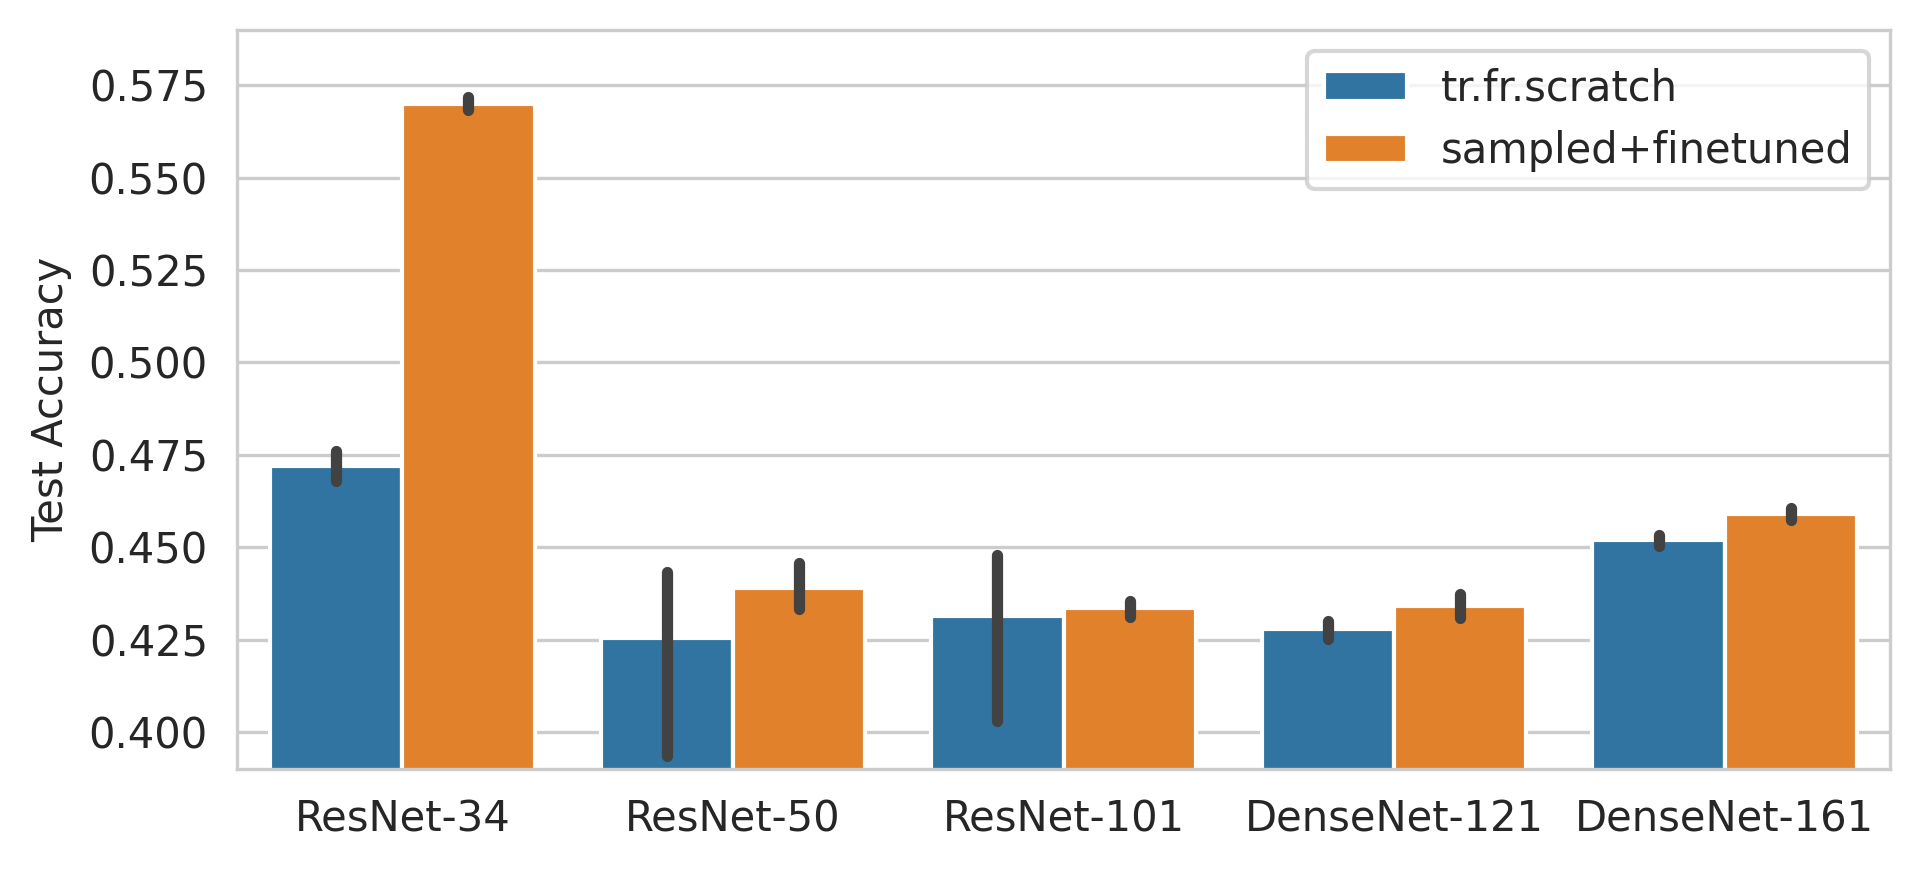
\includegraphics[trim=0mm 0mm 0mm 0mm, width=1.0\linewidth]{figures/sample_accross_architectures_bar_2.png}
\vspace{-2mm}
\captionof{figure}{Comparison between sampled models and random initialization trained for 5 epochs Tiny-Imagenet. Different architectures are sampled from \ourmethod pretrained on a ResNet-18 CIFAR-100 zoo. Although both models and tasks are changed, sampled models perform better.}
\label{fig:sampling_new_arch_task}    
\end{figure}
%%%%%%%%%%%%


\subsection*{Limitations}
In this paper, we pretrain \ourmethod on homogeneous zoos with one architecture. This simplifies alignment for pre-training, but more importantly it simplifies evaluation for model generation. Since \ourmethod can train on varying architectures and model sizes, the model population requirement for pre-training is significantly relaxed. A sufficient number of models are available on public model hubs. 
Further, our sampling method requires access to prompt examples, to have an informed prior from which to sample. For small models, bootstrapping from a Gaussian finds the targeted distribution; see \ourmethod$_{GAUSS}$ in Table \ref{tab:generative_cnn_zoos_in_domain}. For large models with correspondingly long sequences, that approach is too expensive, which is why we rely on prompt examples.  
Lastly, in this paper, we perform experiments only on computer vision tasks. This is a choice to simplify the experiment setup.
%%%%%%%%%%%%%%%%%%%%%%%%%%%%%%%%%%%%%%%%%%%%%%%%%%%%%%%%%%%%%%%%%%%%%%%%%%%%%%%%%

